\begin{figure*}[t]
\centering
\begin{subfigure}[t]{0.45\textwidth}
\centering
\resizebox{\linewidth}{!}{%
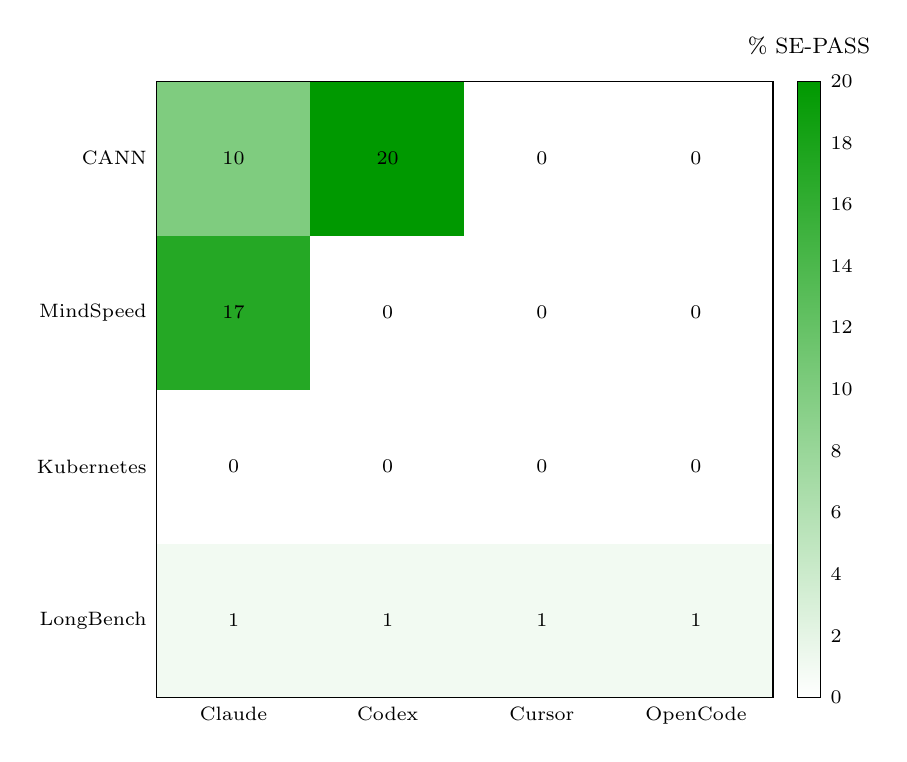
\begin{tikzpicture}
\begin{axis}[
    colormap={gr}{color=(white) color=(green!60!black)},
    colorbar,
    colorbar style={width=3mm, title={\footnotesize \% SE-PASS}, yticklabel style={font=\scriptsize}},
    point meta min=0, point meta max=20,
    xtick={0,1,2,3},
    xticklabels={Claude, Codex, Cursor, OpenCode},
    ytick={0,1,2,3},
    yticklabels={LongBench, Kubernetes, MindSpeed, CANN},
    tick style={draw=none},
    axis on top,
    enlargelimits=false,
    axis equal image,
    width=0.9\linewidth,
    xticklabel style={font=\scriptsize},
    yticklabel style={font=\scriptsize},
    nodes near coords,
    nodes near coords style={font=\scriptsize},
    nodes near coords align=center,
    point meta=explicit,
  ]
    \addplot[
      matrix plot*,
      mesh/cols=4,
      point meta=explicit,
      shader=flat corner,
    ] table[row sep=\\, meta=v] {
      x y v\\
      0 0 1\\
      1 0 1\\
      2 0 1\\
      3 0 1\\
      0 1 0\\
      1 1 0\\
      2 1 0\\
      3 1 0\\
      0 2 17\\
      1 2 0\\
      2 2 0\\
      3 2 0\\
      0 3 10\\
      1 3 20\\
      2 3 0\\
      3 3 0\\
    };
  \end{axis}
\end{tikzpicture}}
\caption{SE-PASS heatmap by family and agent.}
\label{fig:pass-heatmap}
\end{subfigure}\hfill
\begin{subfigure}[t]{0.45\textwidth}
\centering
\resizebox{\linewidth}{!}{%
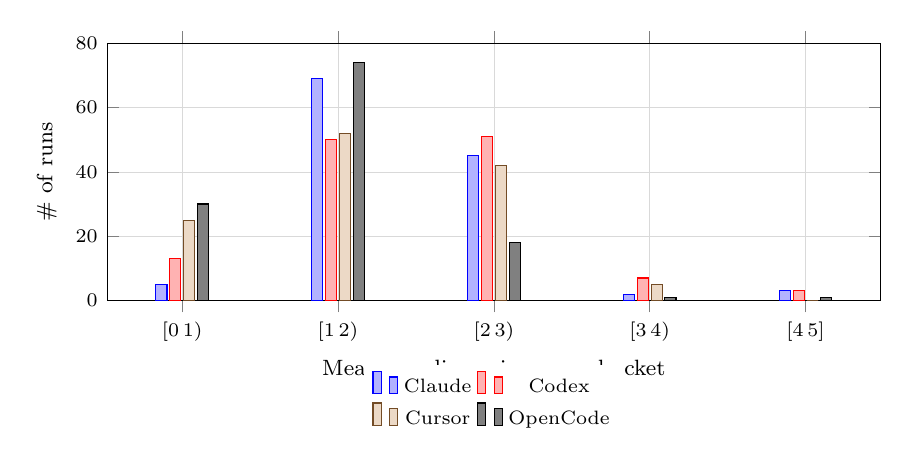
\begin{tikzpicture}
\begin{axis}[
  width=0.94\linewidth,
  height=4.85cm,
  ybar=1pt,
  bar width=4pt,
  symbolic x coords={[0\,1),[1\,2),[2\,3),[3\,4),[4\,5]},
  xtick=data,
  xlabel={\footnotesize Mean per-dimension score bucket},
  ylabel={\footnotesize \# of runs},
  ymin=0, ymax=80,
  enlarge x limits=0.12,
  legend style={font=\scriptsize, at={(0.5,-0.25)}, anchor=north, draw=none, legend columns=2},
  tick label style={font=\scriptsize},
  label style={font=\scriptsize},
  grid=both,
  major grid style={line width=0.2pt, draw=gray!30},
  minor tick num=0,
]
\addplot coordinates {([0\,1),5) ([1\,2),69) ([2\,3),45) ([3\,4),2) ([4\,5],3)};
\addplot coordinates {([0\,1),13) ([1\,2),50) ([2\,3),51) ([3\,4),7) ([4\,5],3)};
\addplot coordinates {([0\,1),25) ([1\,2),52) ([2\,3),42) ([3\,4),5) ([4\,5],0)};
\addplot coordinates {([0\,1),30) ([1\,2),74) ([2\,3),18) ([3\,4),1) ([4\,5],1)};
\legend{Claude, Codex, Cursor, OpenCode}
\end{axis}
\end{tikzpicture}}
\caption{Per-run score distribution by agent.}
\label{fig:score-histogram}
\end{subfigure}
\vspace{-0.4em}
\caption{Result diagnostics. Panel~(a) shows that SE-PASS outcomes concentrate in bounded CANN/MindSpeed tasks and the single LongBench outlier, while Kubernetes remains at 0\%. Panel~(b) shows that most runs occupy the low-to-mid score buckets, explaining why mean-score gains often indicate better drafts rather than merge-ready PRs.}
\Description{Two-panel figure. The first panel is a heatmap of SE-PASS rates by agent and task family. The second panel is a grouped histogram of per-run mean score buckets for the four agents.}
\label{fig:result-diagnostics}
\end{figure*}
